\documentclass[english,11pt]{article}
\usepackage[T1]{fontenc}
\usepackage[utf8]{inputenc}
\usepackage{graphicx}
\usepackage{bm}
\usepackage{geometry}
\usepackage{caption}
\usepackage{subcaption}
\usepackage{babel}
\usepackage{amsmath}
\usepackage[nottoc,numbib]{tocbibind}
\usepackage{verbatim}
\usepackage{hyperref}
\numberwithin{equation}{section}
\newcommand{\naive}{na\"{\i}ve\ }
\newcommand{\Naive}{Na\"{\i}ve\ }

\begin{document}

\title{Machine Learning 4 Assessed Exercise}
\author{Motiejus Jakštys}
\date{28 February 2013}

\maketitle
\pagebreak
\tableofcontents
\pagebreak

\section{Introduction}
\subsection{Identification}
This document is the report of the Machine Learning 4 Assessed Exercise.

\subsection{Contents of the deliverable}

This deliverable is a report of the assessed exercise. It includes the task
description, model, design of the application and performance evaluation.

\subsection{High-level overview of problem and solution}

\subsubsection{Problem description}

When user operates a touch-screen device, she is likely to touch inexact
locations\cite{WeiRogMur}. Errors are not random, which means that, given some
training data, the pointing accuracy can be improved.

The problem can be tackled by creating user a specific model for her touch
behaviour and applying a machine learning technique, which can infer the
intended touch location from the one reported by the device using the training
data.

For mechanism to work it needs a set of locations where the user intended to
touch alongside where the user actually touched, reported by the device. That
can be achieved by a game or some other more or less intrusive way, which is out
of the scope of this document.

This report describes a machine-learning approach, which solves the problem of
adjusting the real touch values provided by the device. In highest level it
learns user behaviour by having some training touch data (300 touches per user),
and then, given a new set of touch coordinates, returns an inferred touch
location.

The approach adopted in this work is Gaussian Process, which is described in
more detail in~\cite{WeiRogMur}.

\section{Model}

The was hard to fit to a "standard" prediction model (for example, linear
or polynomial regression) because of the fact that every touch has two points,
which are dependent. On the same side we do not want to make strong predictions,
like these data are independent, so a more complex model is needed.

Paper~\cite{WeiRogMur} claims it is accurate enough for this particular task,
which was one of the final reason for choosing this model.

Detailed information about Gaussian Processes can be found here~\cite{GP}.

\subsection{Gaussian Process(GP) machinery}

\newcommand{\z}{\textrm{\bf{\v{z}}}}
\newcommand{\zn}{\textrm{\bf{\v{z}$_n$}}}
\newcommand{\zm}{\textrm{\bf{\v{z}$_m$}}}

Here is a brief walkthrough of the steps that were implemented in order to get
the prediction required.

$x^*$ and $y^*$ are values that should be inferred. Further in the paper a
vector $\z = [x, y]^T$ where $x$ and $y$ are touch values reported by the
device.

The goal is Gaussian
distribution of $x^*$ and $y^*$:

$$ (x^*, y^*) \sim \mathcal{N}(\bm{\mu}, \bm{\Psi}) $$

Where

$$ \bm{\mu} = \hat{\textrm{\bf{c}}} [ \hat{\textrm{\bf{C}}} +
    \sigma^2 \textrm{\bf{I}} ]^{-1} \textrm{\bf{z}}
$$

$\bm{\mu}$ is the mean and $\bm{\Psi}$ is the variance. Since confidence of
prediction is not necessary, this value will not be calculated.

GP needs covariance function to work, which defines how similar $\zn$ and $\zm$
inputs are. It is defined as:

$$ C(\zn, \zm) = b(a \zn^T\zm +
(1 - a)e^{-\gamma || \zn - \zm ||^2 } )
$$

For details of the meaning of $a$, $b$, $\gamma$, refer to
paper~\cite{WeiRogMur}. This paper is concerned how to optimize them for best
prediction performance.

\subsection{Implementation details}

Paper~\cite{WeiRogMur} defines the rest of machinery neatly enough and in a very
compact manner, so rest of the machinery is left out of this paper. However,
there are some things to note.

$b$, $a$, $\gamma$, $\sigma^2$ are free parameters that have to be pre-set,
ideally using cross-validation. What is more, paper~\cite{WeiRogMur} provides
their initial values: $a = 0.1$, $\alpha = 0.9$, $\sigma^2 = 0.001$, $\gamma =
0.05$, $b = 5$. In order to achieve slightly better results than the original
paper, cross-validation with different values of these parameters was performed.
In the end for this data set, these values yield slightly best results: $a =
0.1$, $b = 10$, $\alpha = 0.9$, $\sigma^2 = 0.001$.

\section{Result analysis}

Variables $a$ and $b$ were varied using 10-fold analysis.
Figure~\ref{fig:error_a} shows root mean square of error mean per user with
varying $a$. Equivalently figure~\ref{fig:error_b} for $b$. This shows quite
good indication that $a$ should be $0.1$ and $b$ should be $10$.

In future work it would be useful to test influence of $\gamma$.  Intuitively,
$\sigma^2$ will not yield better performance, but in $\gamma$ case we can expect
anything.

\begin{figure}
    \centering
    \begin{subfigure}[b]{0.8\textwidth}
        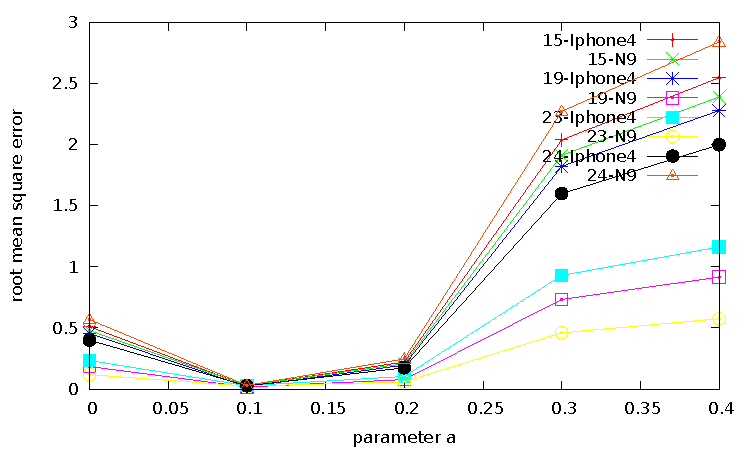
\includegraphics[width=\textwidth]{error_a}
        \caption{RMS error varying $a$}
        \label{fig:error_a}
    \end{subfigure}

    \begin{subfigure}[b]{0.8\textwidth}
        \caption{RMS error varying $b$}
        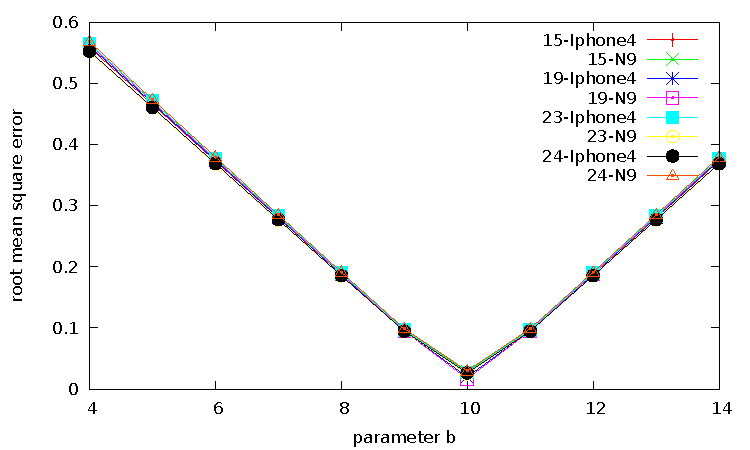
\includegraphics[width=\textwidth]{error_b}
        \label{fig:error_b}
    \end{subfigure}
    \caption{RMS errors with varying parameters}\label{fig:aggr}
\end{figure}


\section{Conclusions}
This paper describes machine learning approach based on GP regression in order
to increase user specific touch accuracy, and that varying free parameters in GP
can make really big difference.

However, the greatest achievement of the exercise is a working GP regression
implementation with (subjectively) quite decent performance.

\begin{thebibliography}{9}

    \bibitem{WeiRogMur}
        Daryl Weir, Simon Rogers, Markus L\"ochtefeld, and Roderick
        Murray-Smith. A user-specific machine learning approach for improving
        touch accuracy on mobile devices. \emph{In Proceedings of the 25th ACM
        Symposium on User Interface Software and Technology}, 2012.

    \bibitem{GP}
        Rasmussen, C. E., and Williams, C. K. I. \emph{Gaussian Processes for
        Machine Learning}. MIT Press, 2006.

\end{thebibliography}
\end{document}
